\documentclass[10pt]{article}
\usepackage[utf8]{inputenc}
\usepackage{url}
\usepackage[table]{xcolor}
\usepackage{graphicx}
\usepackage{blindtext}
\usepackage{enumitem}
\usepackage{booktabs}

\title{First document}
\author{Group 3}
\date{October 2018}

\begin{document}


\section{Description and Demonstration of Modules}
This document intends to thoroughly explain the implementation of the important modules and functions of the system.

\subsection{Form Modules}
The main thing we want to do on our website is create a nice way to add and edit blog posts. With forms we will have absolute power over our interface – we can do almost anything we can imagine!

\subsubsection{AVI Module Forms}
We use Django built in form creator to create a basic form which will then have to pass our required attributes(which invoke database usage- to be discussed later) to it - ‘from Django import forms’.

\subsubsection{The Django Form class}
At the heart of this system of components is Django’s Form class. In much the same way that a Django model describes the logical structure of an object, its behavior, and the way its parts are represented to us, a Form class describes a form and determines how it works and appears.

\subsubsection{Django’s role in forms}

Handling forms is a complex business. Consider Django’s admin, where numerous items of data of several different types may need to be prepared for display in a form, rendered as HTML, edited using a convenient interface, returned to the server, validated and cleaned up, and then saved or passed on for further processing.

Django’s form functionality can simplify and automate vast portions of this work, and can also do it more securely than most programmers would be able to do in code they wrote themselves.

Django handles three distinct parts of the work involved in forms:

\begin{description}[font=$\bullet$~\normalfont\scshape\color{red!50!black}]
\item [] preparing and restructuring data to make it ready for rendering.
\item [] creating HTML forms for the data.
\item [] receiving and processing submitted forms and data from the client.
\end{description}

It is possible to write code that does all of this manually, but Django can take care of it all for you.

We link the form attributes to the models (database tables) pre-defined under the models python file of the app. This allows user input options and verification of requests inputs.

\subsubsection{Avi App Form Functions}
The Create User Form: Extracted from “avi\_app/forms.py”

\begin{center}
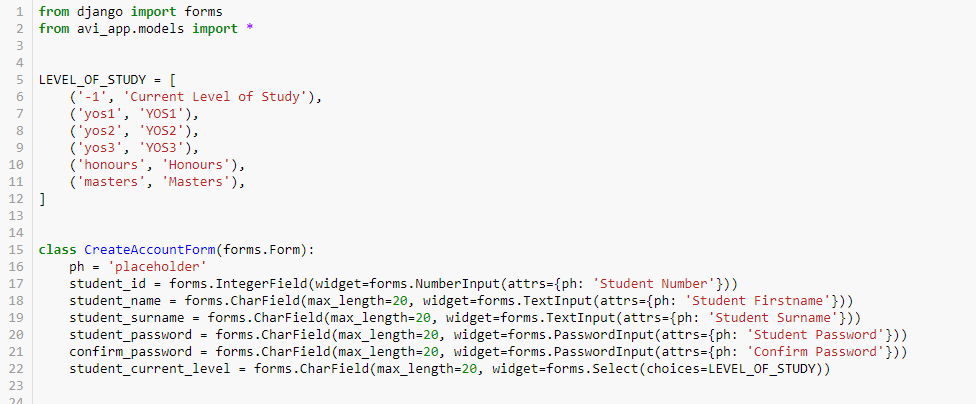
\includegraphics[width=.9\textwidth]{forms.png}
\end{center}
\caption{\underline{forms.py}} \\ \\

The class ’CreateAccountForm(form.Form)’ instantiates the Student Class attributes therefore enabling them to be used in the form. We specify the type of input we can expect for each attribute which enables us to check whether the user input is valid. This class is used in incorporation with html code and CSS for the createaccount.html file. 

This form allows users to register to use the website app. This is what final form looks like:

\begin{center}
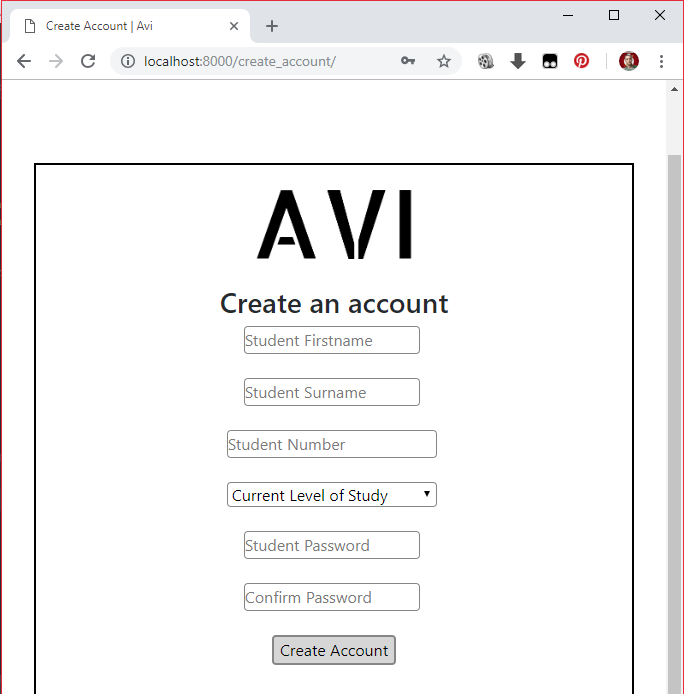
\includegraphics[width=.4\textwidth]{create_A.png}
\end{center}
\caption{\underline{create account}}

\subsubsection{The Login Form}

The following lines of code instantiates the login form attributes. This form allows user to be able to login to the website app.

\begin{center}
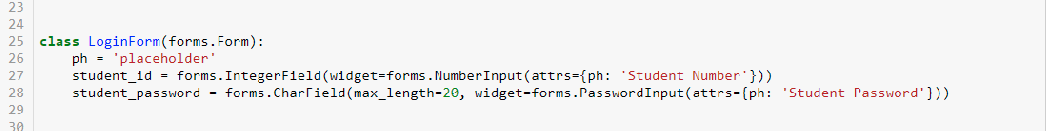
\includegraphics[width=.9\textwidth]{login_form.png}
\end{center}
\caption{\underline{Login Form}} \\ \\

This along with the html and CSS code leads to the following form being created:

\begin{center}
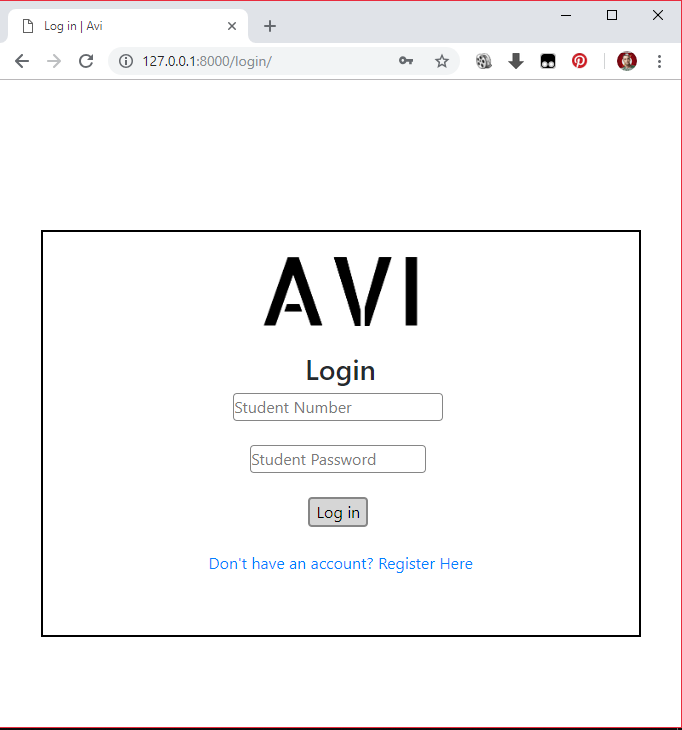
\includegraphics[width=.4\textwidth]{login_page.png}
\end{center}
\caption{\underline{Login}} \\ \\

\subsubsection{Add Courses Form}
Extracted from “avi\_app/forms.py”.

This form allows users to be add courses to their profile.

\begin{center}
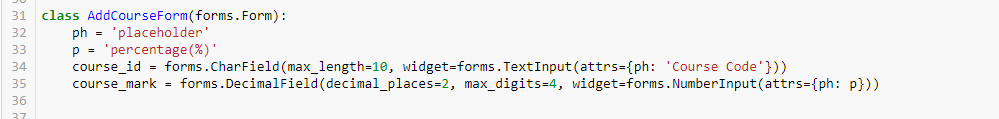
\includegraphics[width=.9\textwidth]{add_course.png}
\end{center}
\caption{\underline{Add Course}} \\ \\

The above code along with the html and CSS code leads to the following form being created:

\begin{center}
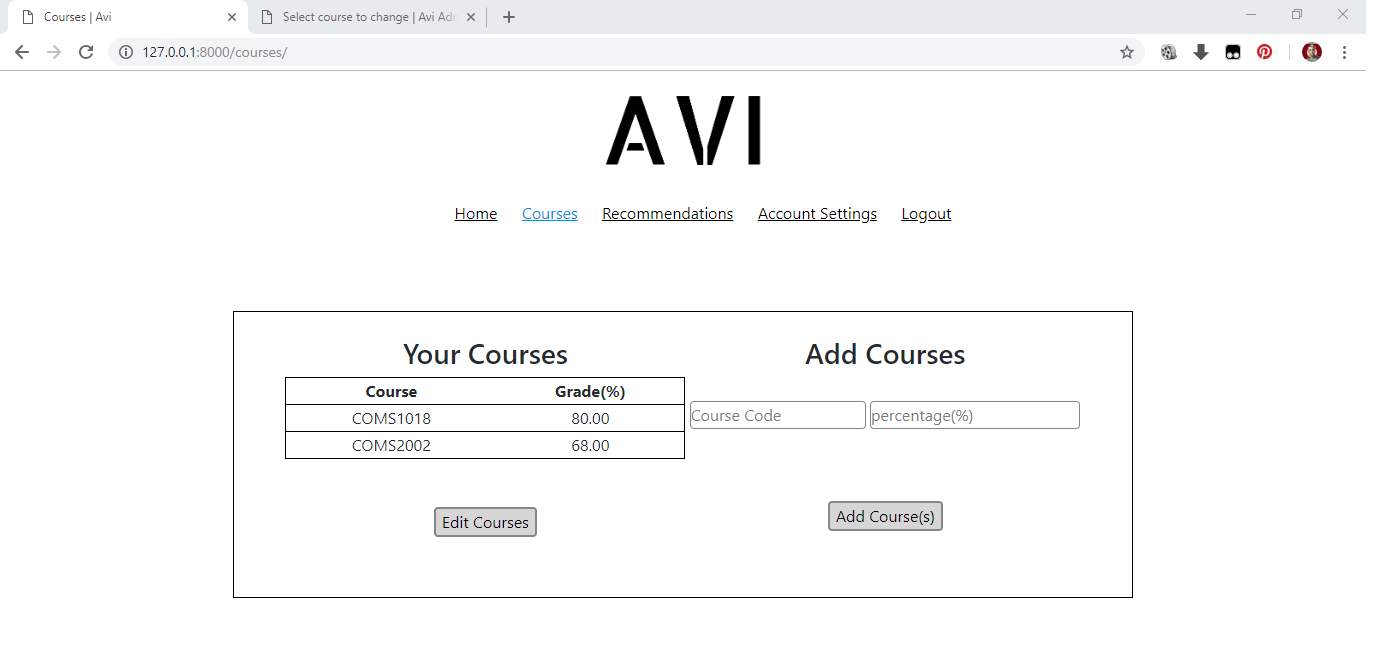
\includegraphics[width=.9\textwidth]{course.png}
\end{center}
\caption{\underline{Course}}

\subsubsection{The  Account Settings Form}

Extracted from “avi\_app/forms.py”.

The following lines of code instantiates foreign key attributes. This form allows user to be able to edit their personal details in the website app.

\begin{center}
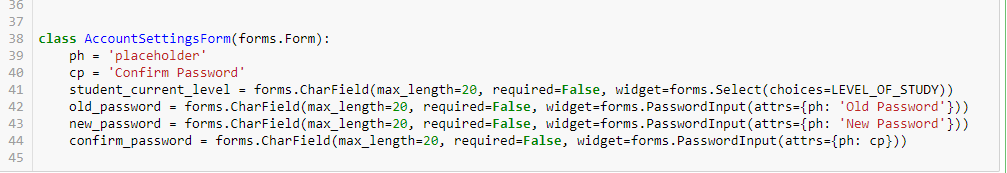
\includegraphics[width=.9\textwidth]{Aform.png}
\end{center}
\caption{\underline{Account Settings}} \\ \\

The above code along with the html and CSS code leads to the following form being created:

\begin{center}
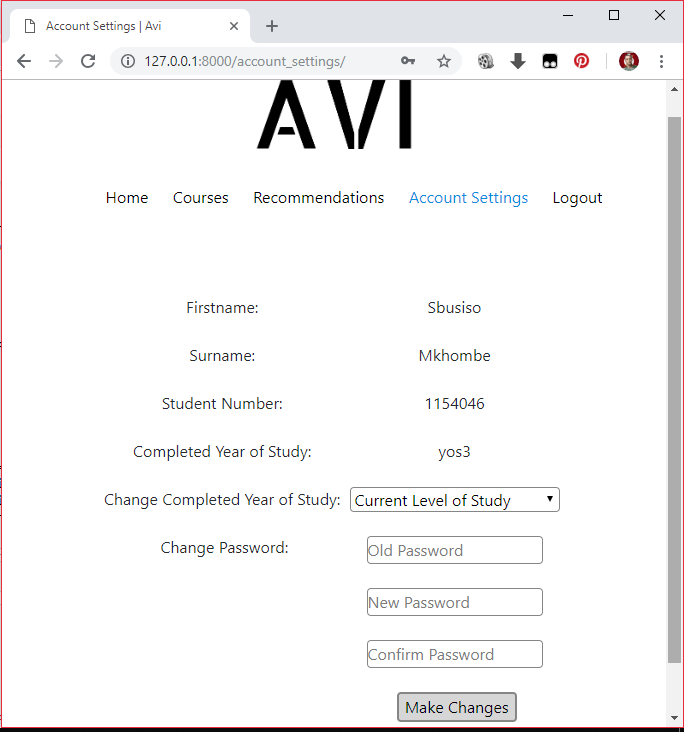
\includegraphics[width=.4\textwidth]{settings.png}
\end{center}
\caption{\underline{Settings}}

\subsection{Models}

Also known as model attributes. A model is the single, definitive source of information about your data. It contains the essential fields and behaviors of the data you’re storing. Generally, each model maps to a single database table.

Once you have defined your models, you need to tell Django you’re going to use those models. Do this by editing your settings file and changing the INSTALLED\_APPS setting to add the name of the module/ app that contains your models.py.

The most important part of a model – and the only required part of a model – is the list of database fields it defines. Fields are specified by class attribute. Examples of fields in our Student Model (Below) would be student\_name, student\_surname and student\_id.

Each field takes a certain set of field-specific arguments (documented in the model field reference). For example, CharField (and its subclasses) require a max\_length argument which specifies the size of the VARCHAR database field used to store the data.There’s also a set of common arguments available to all field types. All are optional.

\subsubsection{Registering our Models}
Django comes with an admin.py file which allows us to register our model - basically add tables to our database.

We register our tables with the following code:

\begin{center}
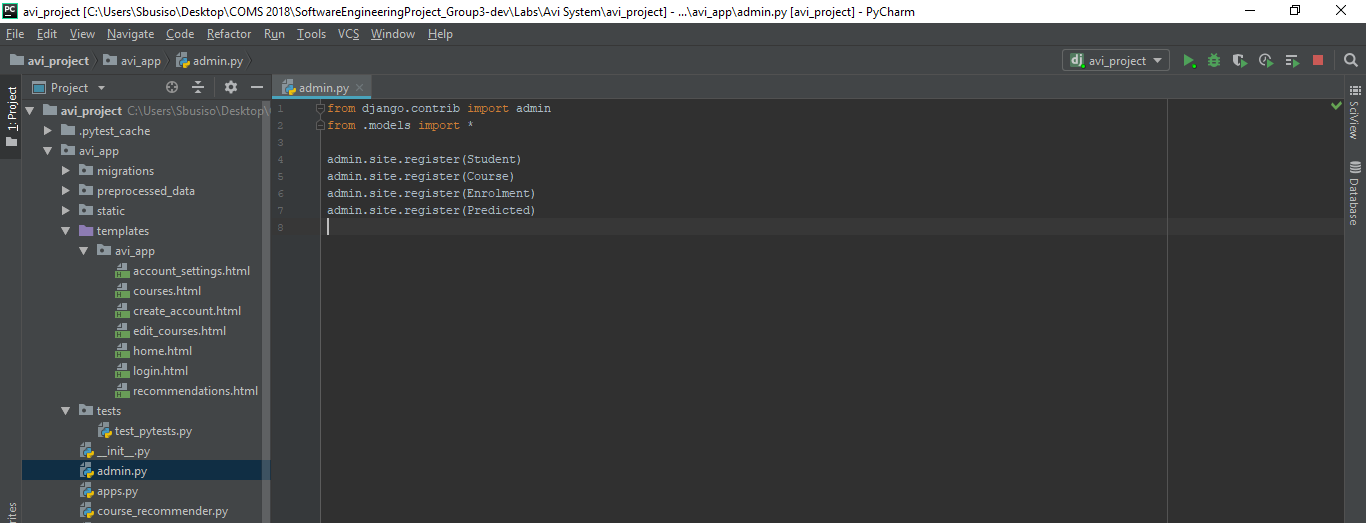
\includegraphics[width=1.1\textwidth]{p1.png}
\end{center} \\ \\

We then use the following commands from our shell to save our database changes:

python manage.py makemigrations avi\_app

python manage.py migrate \\

Defining and initializing our models(tables):

\begin{center}
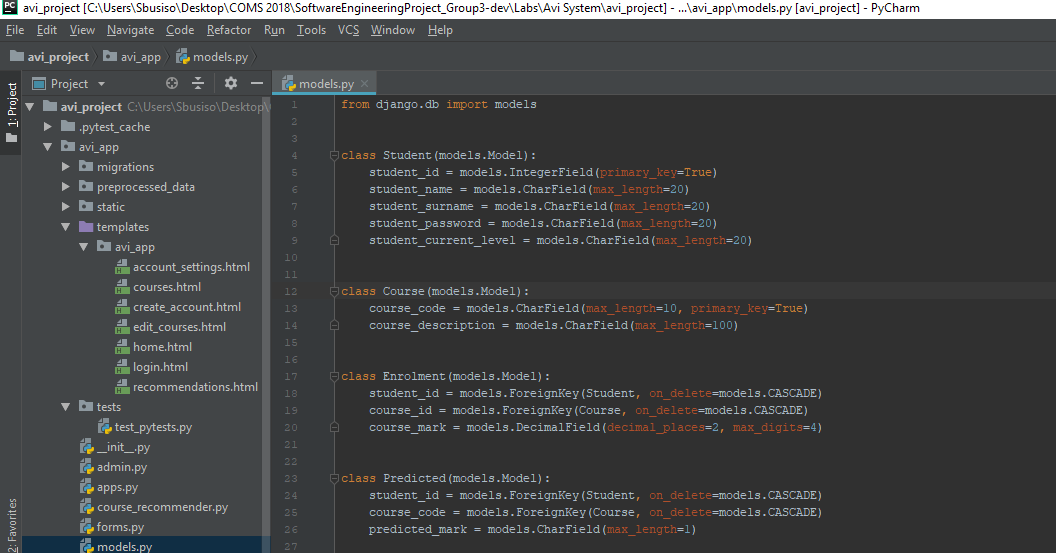
\includegraphics[width=1.1\textwidth]{p2.png}
\end{center} \\ \\

 
The shell migration command leads to these tables being created:

(These can be accessed from http://127.0.0.1:8000/admin with the admin as username and “pass1234” as password for admin access).

\begin{center}
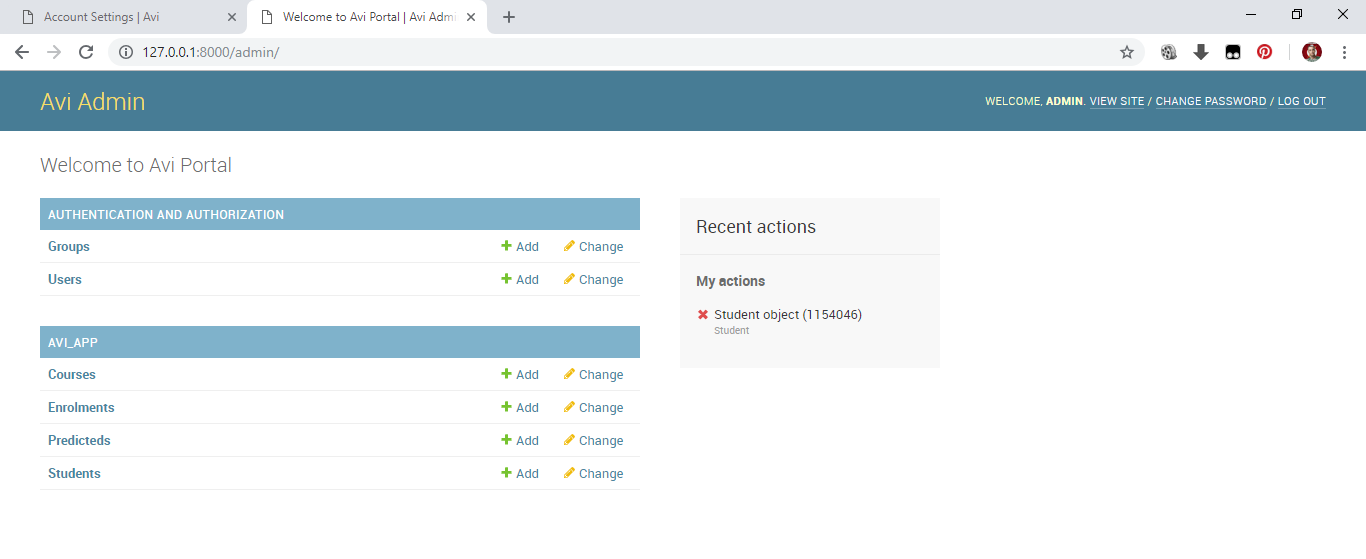
\includegraphics[width=1.1\textwidth]{p3.png}
\end{center} \\ \\

\subsubsection{Django URL  Dispatcher}

A clean, elegant URL scheme is an important detail in a high-quality Web application. Django lets you design URLs however you want, with no framework limitations.

To design URLs for an app, you create a Python module informally called a URLconf (URL configuration). This module is pure Python code and is a mapping between URL path expressions to Python functions (your views).

This mapping can be as short or as long as needed. It can reference other mappings. And, because it’s pure Python code, it can be constructed dynamically.

\subsubsection{How Django processes a request}

When a user requests a page from your Django-powered site, this is the algorithm the system follows to determine which Python code to execute:

\begin{description}[font=$\bullet$~\normalfont\scshape\color{red!50!black}]

\item [] Django determines the root URLconf module to use. Ordinarily, this is the value of the ROOT\_URLCONF setting, but if the incoming HttpRequest object has a urlconf attribute (set by middleware), its value will be used in place of theROOT\_URLCONF setting.

\item [] Django loads that Python module and looks for the variable urlpatterns. This should be a Python list of django.urls.path() and/or django.urls.re\_path() instances.

\item [] Django runs through each URL pattern, in order, and stops at the first one that matches the requested URL.

\item [] Once one of the URL patterns matches, Django imports and calls the given view, which is a simple Python function (or a class-based view). The view gets passed the following arguments:

 \SubItem{- An instance of HttpRequest.}
 
 \SubItem{- If the matched URL pattern returned no named groups, then the matches from the regular expression are provided as positional arguments.}
 
 \SubItem{- The keyword arguments are made up of any named parts matched by the path expression, overridden by any arguments specified in the optional kwargs argument to django.urls.path() or django.urls.re\_path().}

\item [] If no URL pattern matches, or if an exception is raised during any point in this process, Django invokes an appropriate error-handling view.
\end{description}

From “avi\_app/urls.py”:

We initialize all urls we want our site to expect, for example localhost:8000/login would be a valid url because we have declared it in line 8.

\begin{center}
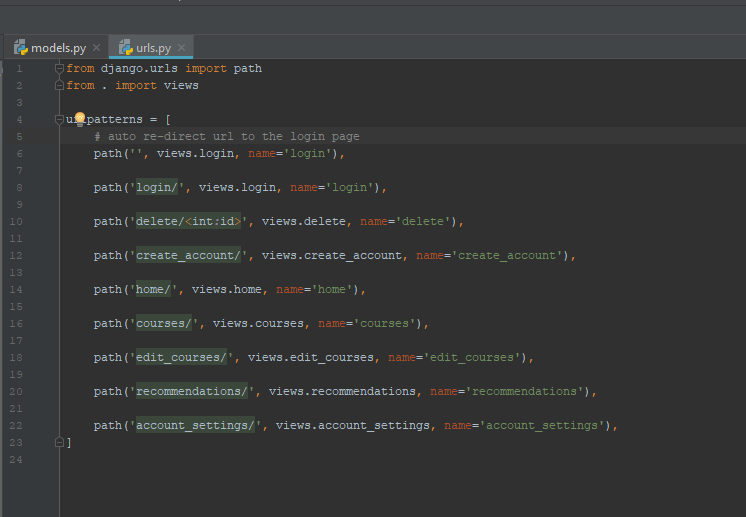
\includegraphics[width=1.1\textwidth]{p4.png}
\end{center} \\ \\

Line 8 declares the path/url that localhost:8000/login redirects to – views.login then ensures that the login method in the views.py file is associated with this url and used in its execution. \\

“from . import views “ – allows us to use methods from our views.py file which are then translated to html files and forms which are then displayed to the user. \\

We declare our overall usage of urls in our main url file url.py in line 12 by basically declaring the inclusion of all the other urls in the avi\_app.

\begin{center}
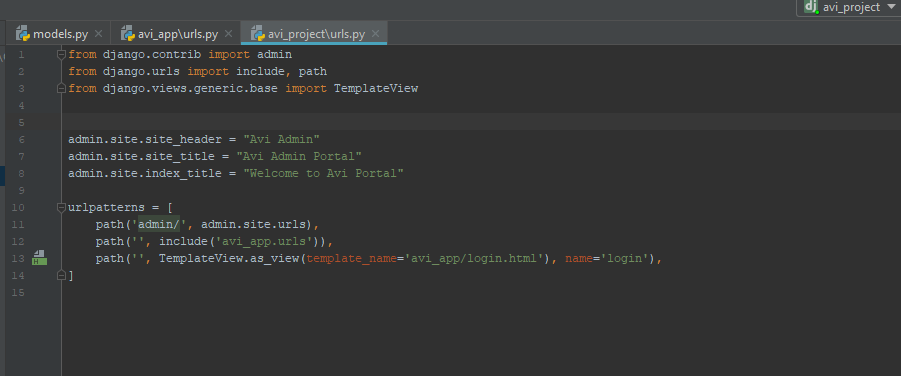
\includegraphics[width=1.1\textwidth]{p5.png}
\end{center} \\ \\

\subsection{Views}

\subsubsection{Create Account Module}

\begin{center}
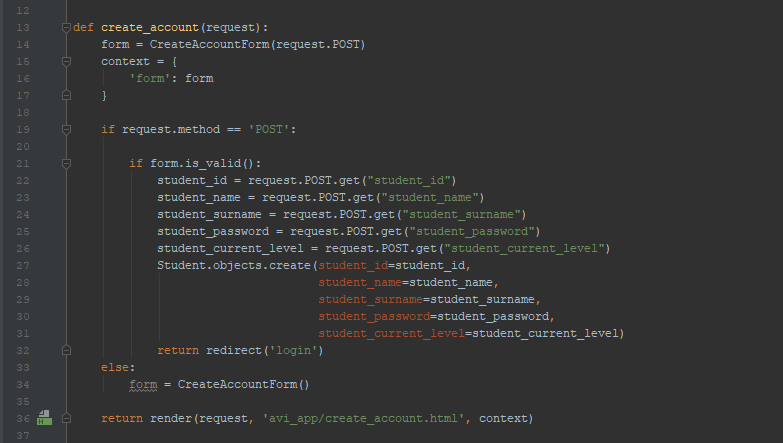
\includegraphics[width=1.1\textwidth]{p6.png}
\end{center} \\ \\

\begin{description}[font=$\bullet$~\normalfont\scshape\color{red!50!black}]
\item [] This module is essential in the create account form functionality. 
\item [] It creates a form instance to display (line 13-17).
\item [] Checks if the user is attempting to fill data into the form (line 19).
\item [] If yes, checks if user has submitted valid input to the form (line 21).
\item [] If the form is valid, it then creates and stores the data into variables.
\item [] A student object is then stored in our database table which uses the variables we declared as column attributes.
\item [] It then redirects us to the login page where we are then able to login with our credentials.

\end{description}

\subsubsection{Login Module}

\begin{center}
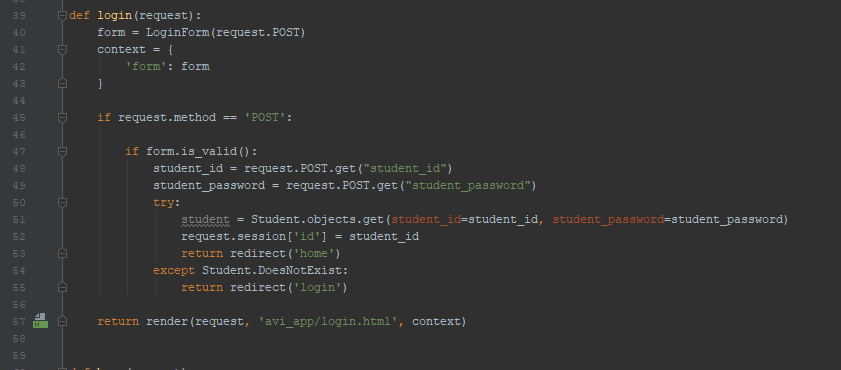
\includegraphics[width=1.1\textwidth]{p7.png}
\end{center} \\ \\

\begin{description}[font=$\bullet$~\normalfont\scshape\color{red!50!black}]
\item [] This module is essential in the create account form functionality. 
\item [] It creates a form instance to display (line 40-43).
\item [] Checks if the user is attempting to fill data into the form (line 45).
\item [] If yes, checks if user has submitted valid input to the form (line 47).
\item [] If the form is valid, it then creates variables which are used for authentication by checking if they match the values of the corresponding attribute in our database. (line 50-52).
\item [] If they do, the student is then logged-in and redirected to the home screen. (line 53).
\item [] Else they have to try logging in again. (line 54-55).

\end{description}

\subsubsection{Home Module}

\begin{center}
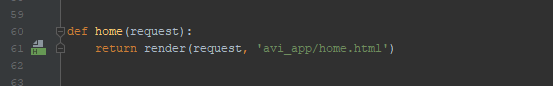
\includegraphics[width=1.1\textwidth]{p8.png}
\end{center} \\ \\

This module redirects the request to the homepage when used in urls.


\subsubsection{Course Module}

\begin{center}
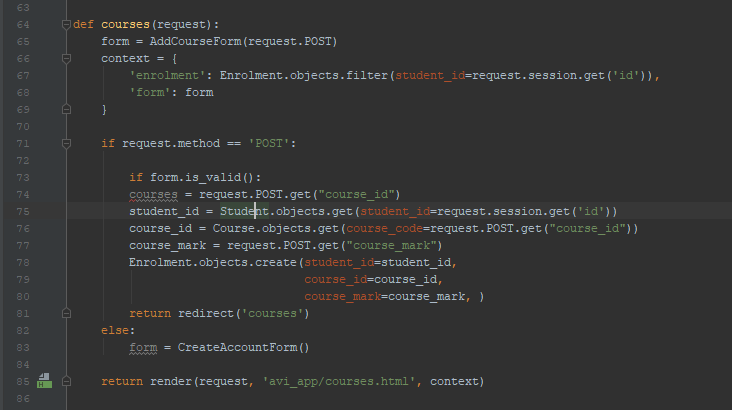
\includegraphics[width=1.1\textwidth]{p9.png}
\end{center} \\ \\

\begin{description}[font=$\bullet$~\normalfont\scshape\color{red!50!black}]
\item [] This module is essential in the adding courses form functionality. 
\item [] It creates a form instance to display (line 65-69).
\item [] Checks if the user is attempting to fill data into the form (line 71).
\item [] If yes, checks if user has submitted valid input to the form (line 73).
\item [] If the form is valid, it then creates and stores the data into variables.
\item [] A course object is then stored in our database table which uses the variables we declared as column attributes.
\item [] It then redirects us to the courses page where we are then able to see our added courses.
\item [] If the form info passed is invalid, the form is recreated (line 83) and the user can retry adding his or her courses. (line 85).

\end{description}

\subsubsection{Edit Courses Module}

\begin{center}
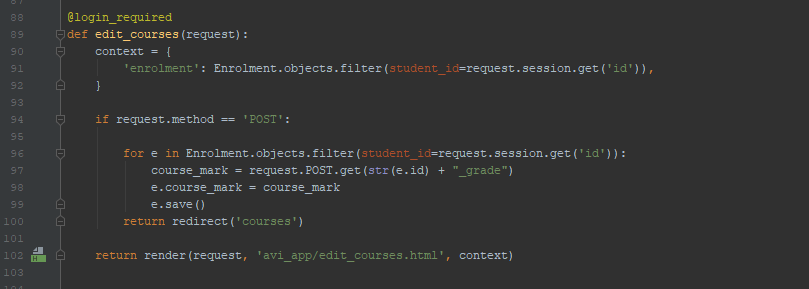
\includegraphics[width=1.1\textwidth]{p10.png}
\end{center} \\ \\

\begin{description}[font=$\bullet$~\normalfont\scshape\color{red!50!black}]
\item [] Line 88 declares that login is required for user to be able to access this view (form). This method is extracted from the  from the Django contrib.auth class and we import the login required from it. (check imports).
\item [] Line 90 – 92 we define the form context and filter ‘student\_id’ to ensure that the request is from a valid student-object (user). 
\item [] We then check if the user is trying to pass input to the form (Line 94).
\item [] If yes, we then iterate through the enrolment table for the user and update their marks for every updated mark input they pass.
\item [] e.save() achieves this for every updated mark input. (Line 99).
\item [] The user is then redirected to the courses page which now displays all their updated marks.
\item [] If the user has passed invalid input or no input at all, they are redirected to the edit courses page and given a new form to try updating their course or course mark again.

\end{description}

\subsubsection{Delete  Module}


\begin{center}
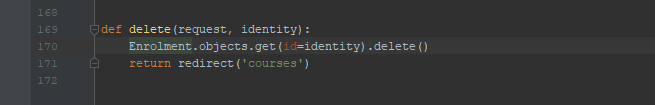
\includegraphics[width=1.1\textwidth]{p11.png}
\end{center} \\ \\

\begin{description}[font=$\bullet$~\normalfont\scshape\color{red!50!black}]
\item [] The delete courses module deletes a user course from our database.
\item [] The course id is passed as identity into the function and the corresponding course is deleted from the user’s courses.
\item [] The courses view is then updated accordingly.

\end{description}

\subsubsection{Recommendations Module}

\begin{center}
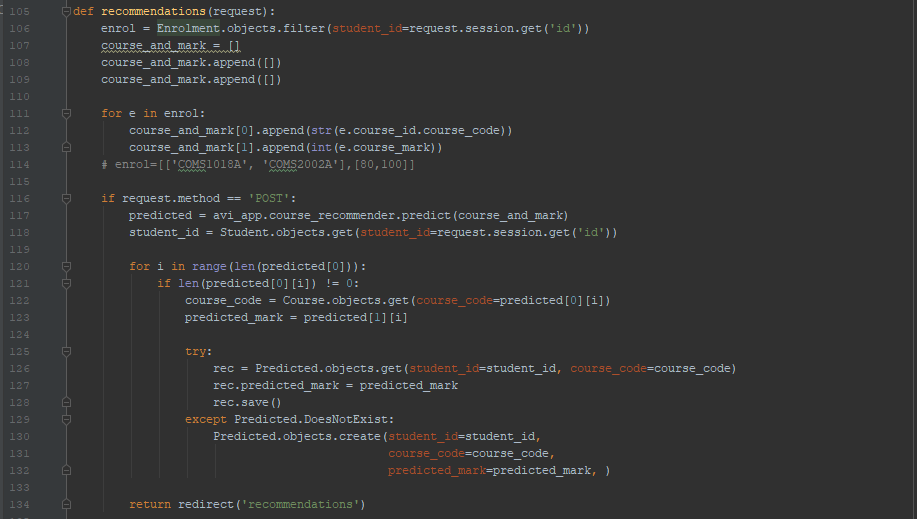
\includegraphics[width=1.1\textwidth]{p12.png}
\end{center} \\ \\



\begin{description}[font=$\bullet$~\normalfont\scshape\color{red!50!black}]
\item [] We redefine a new enrolment called enrol which ensures that user is logged in.(Line 106). 
\item [] We define a new python list variable called course and mark which will store a course and its corresponding mark.
\item [] A for-loop is used to append the users courses and marks into the list. (line 111-113).
\item [] A check is used to ensure that the user is trying to get recommendations. (line 116).
\item [] We use the course\_recommender module from recommender.py to get our final recommendations for courses.
\item [] An if statement is used to check that our courses marks list is not empty, if not we then return the predicted marks for their respective courses.
\item [] The recommendations are then returned to the student through the recommendations view( Line 134).

\begin{center}
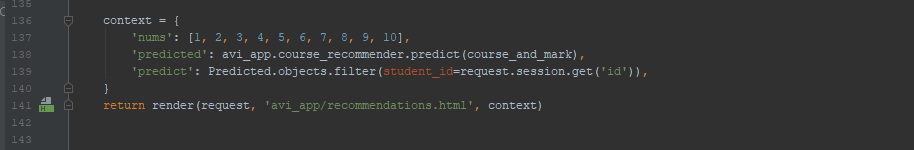
\includegraphics[width=1.1\textwidth]{p13.png}
\end{center} \\ \\

\item [] If the user didn’t pass valid form values or the form was empty we define a new context.

\item [] We then pass it through the recommendations form which enables the user to try getting  a recommendation again.

\end{description}

\subsubsection{Account Settings Module}

\begin{center}
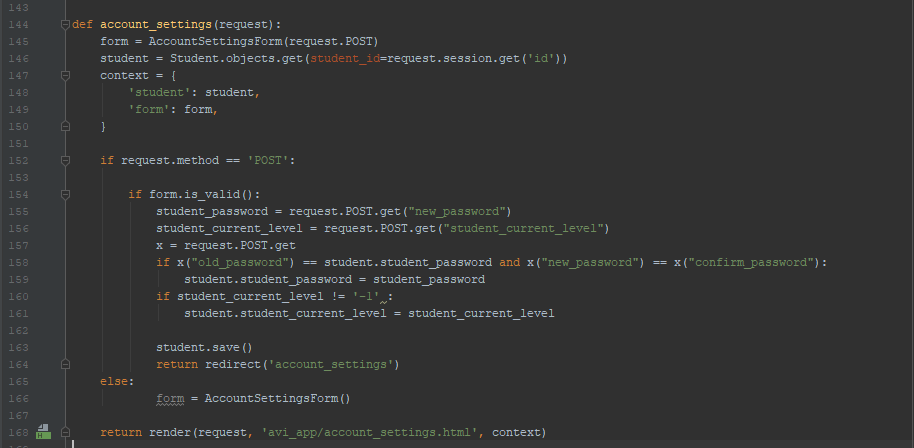
\includegraphics[width=1.1\textwidth]{p14.png}
\end{center} \\ \\

\begin{description}[font=$\bullet$~\normalfont\scshape\color{red!50!black}]
\item [] This module lets the user update their completed year of study and password through the account settings form.
\item [] A form is created which then checks if user is logged in and requires user input - (line 145).
\item [] We define our default context which we will pass to our form to be displayed in our html - (line 147-150).
\item [] We check if the user is attempting to pass input which is valid to our form – (line 152 and 154).
\item [] If the user is attempting to update their current level the new value is stored in the variable ‘student\_current\_level’ - (line 156) and then updated in the database if it’s a valid value – (line 160 and 161). 
\item [] If the user is attempting to update their password, the passed in current password is checked if it matches the one in the database and if valid it changes the password to ‘ new\_password’ value.

\end{description}

\end{document}